



	\documentclass[paper=letter,fontsize=11pt]{scrartcl} % KOMA-article class
\usepackage[english]{babel}
\usepackage[utf8x]{inputenc}
\usepackage[protrusion=true,expansion=true]{microtype}
\usepackage{amsmath,amsfonts,amsthm}     % Math packages
\usepackage{graphicx}                    % Enable pdflatex
\usepackage[svgnames]{xcolor}            % Colors by their 'svgnames'
\usepackage{geometry}
	%\textheight=700px                    % Saving trees ;-)
%\usepackage{url}
\usepackage[colorlinks=true,
linkcolor=blue,
urlcolor=blue]{hyperref}
\usepackage{float}
\usepackage{etaremune}
\usepackage{wrapfig}
\usepackage{framed,graphicx,xcolor}
\definecolor{shadecolor}{rgb}{0.95,0.95,1}

\usepackage{attachfile}

\frenchspacing              % Better looking spacings after periods
\pagestyle{empty}           % No pagenumbers/headers/footers

%\addtolength{\voffset}{-40pt}
%\addtolength{\textheight}{20pt}

\setlength\topmargin{0pt}
\addtolength\topmargin{-\headheight}
\addtolength\topmargin{-\headsep}
\setlength\oddsidemargin{0pt}
\setlength\textwidth{\paperwidth}
\addtolength\textwidth{-2in}
\setlength\textheight{\paperheight}
%\addtolength\textheight{-3in}
\addtolength\textheight{-2in}
\usepackage{layout}

%%% Custom sectioning}{sectsty package)
%%% ------------------------------------------------------------
\usepackage{sectsty}

\sectionfont{%			            % Change font of \section command
	\usefont{OT1}{phv}{b}{n}%		% bch-b-n: CharterBT-Bold font
	\sectionrule{0pt}{0pt}{-5pt}{3pt}}

%%% Macros
%%% ------------------------------------------------------------
\newlength{\spacebox}
\settowidth{\spacebox}{8888888888}			% Box to align text
\newcommand{\sepspace}{\vspace*{1em}}		% Vertical space macro

\newcommand{\MyName}[1]{ % Name
		\Huge \usefont{OT1}{phv}{b}{n} \hfill #1
		\par \normalsize \normalfont}

\newcommand{\MySlogan}[1]{ % Slogan}{optional)
		\large \usefont{OT1}{phv}{m}{n}\hfill \textit{#1}
		\par \normalsize \normalfont}

\newcommand{\NewPart}[2]{\section*{\uppercase{#1} #2}}

\newcommand{\PersonalEntry}[2]{
		\noindent\hangindent=2em\hangafter=0 % Indentation
		\parbox{\spacebox}{        % Box to align text
		\textit{#1}}		       % Entry name}{birth, address, etc.)
		\hspace{1.5em} #2 \par}    % Entry value

\newcommand{\SkillsEntry}[2]{      % Same as \PersonalEntry
		\noindent\hangindent=2em\hangafter=0 % Indentation
		\parbox{\spacebox}{        % Box to align text
		\textit{#1}}			   % Entry name}{birth, address, etc.)
		\hspace{1.5em} #2 \par}    % Entry value

\newcommand{\EducationEntry}[4]{
		\noindent \textbf{#1} \hfill      % Study
		\colorbox{White}{%
			\parbox{10em}{%
			\hfill\color{Black}#2}} \par  % Duration
		\noindent \textit{#3} \par        % School
		\noindent\hangindent=2em\hangafter=0 \small #4 % Description
		\normalsize \par}

\newcommand{\WorkEntry}[4]{				  % Same as \EducationEntry
		\noindent \textbf{#1} \hfill      % Jobname
		\colorbox{White}{\color{White}#2} \par  % Duration
		\noindent \textit{#3} \par              % Company
		\noindent\hangindent=2em\hangafter=0 \small #4 % Description
		\normalsize \par}

\newcommand{\PaperEntry}[7]{
		\noindent #1, ``\href{#7}{#2}", \textit{#3} \textbf{#4}, #5 (#6).}


\newcommand{\ArxivEntry}[3]{
		\noindent #1, ``\href{http://arxiv.org/abs/#3}{#2}", \textit{{cond-mat/}#3}.}

\newcommand{\BookEntry}[4]{
		\noindent #1, ``\href{#3}{#4}", \textit{#3}.}

\newcommand{\FundingEntry}[5]{
        \noindent #1, ``#2", \$#3 (#4, #5).}

\newcommand{\TalkEntry}[4]{
		\noindent #1, #2, #3 #4}

\newcommand{\ThesisEntry}[5]{
		\noindent #1 -- #2 #3 ``#4" \textit{#5}}

\newcommand{\CourseEntry}[3]{
		\noindent \item{#1: \textbf{#2} \\ #3}}

%%% Begin Document
%%% ------------------------------------------------------------
\begin{document}

%\layout

% you can upload a photo and include it here...
\begin{wrapfigure}{l}{0.5\textwidth}
	\vspace*{-2em}
		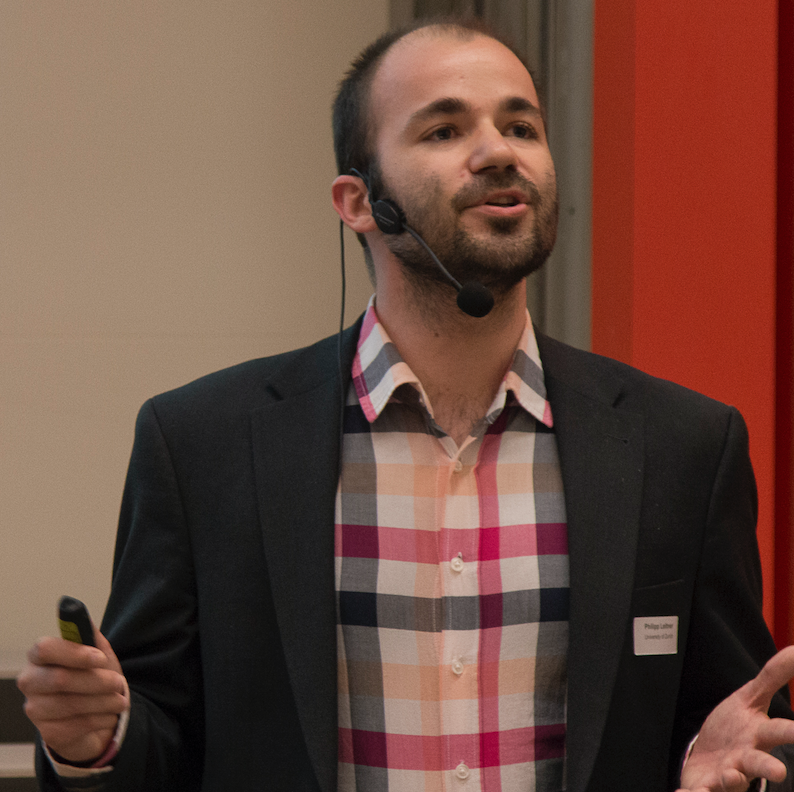
\includegraphics[width=0.18\textwidth]{profile.png}
\end{wrapfigure}

\MyName{Philipp Leitner}
\MySlogan{Curriculum Vit\ae\ (\today)}

\vspace{1cm}

\NewPart{Summary}{}
I am an associate professor (docent) of software engineering at Chalmers University of Technology. I currently lead the Software Engineering 2 unit, focussing on Software Technology. I teach and conduct research on software development tools for Internet-based systems. Recently, much of my research is on software performance engineering, with a special focus on tools that enable rapid releases of efficient cloud software. I currently supervise a team of 4 PhD students working in the above topics, and have graduated three successful students.

My research is funded through WASP, VR, Vinnova, and the Chalmers Area of Advance on ICT. I hold a PhD degree in business informatics from Vienna University of Technology (2011), and have (co-)authored more than 100 publications to date, leading to an h-index of 45 as tracked by Google Scholar. Recent publication highlights include papers at ICSE, FSE, TSE, EMSE, and an an award-winning paper at the USENIX Middleware conference.

In addition to my research and teaching, I organized events (e.g., a Dagstuhl seminar on software performance engineering, or the Vienna Software Seminar series) and special issues related to my area of research. I serve on the programme committee of many of the most visible conferences in the field (e.g., MSR, ICSME, ICPE), and have also acted in organisatorial roles (e.g., PC chair at ICPE in 2022) for various conferences.


%%% Work experience
%%% ------------------------------------------------------------
\NewPart{Recent Appointments}{}
\EducationEntry{Associate Professor}{Since Oct. 19}{Chalmers $|$ University of Gothenburg}{}
\EducationEntry{ICT Area of Advance Assistant Professor (tenure-track)}{Aug. 17 - Oct. 19}{Chalmers University of Technology}{}

\EducationEntry{Senior Research Associate}{Jan. 14 - July 17}{University of
Zurich}{
}
\EducationEntry{Postdoctoral Researcher}{Nov. 2011 - Dec. 2013}{Vienna
University of Technology}{}

\NewPart{Recent Acquired Grants}{}

\renewcommand{\arraystretch}{0.75}
  \begin{tabular}{p{4.8cm}ll}
          \textbf{Debloating ML Systems} & \emph{Funding:} AoA SEED Grant & \emph{Role:} Co-PI \\
    (2021) & & \\
        \textbf{FFI TRAF-Cloud} & \emph{Funding:} Vinnova & \emph{Role:} Co-PI \\
    (2019 - 2022) & & \\
      \textbf{VR Starting Grant} & \emph{Funding:} VR & \emph{Role:} PI \\
    (2019 - 2023) & & \\
      \textbf{WASP Student} & \emph{Funding:} WASP & \emph{Role:} PI \\
    (2017 - 2022) & & \\
      \textbf{MINCA} & \emph{Funding:} SNF (Swiss) & \emph{Role:} PI \\
    (2016 - 2019) & & \\
%    \textbf{DevCloud} & \emph{Funding:} Hasler Foundation (Swiss) & \emph{Role:} Co-PI \\
%    (2016) & & \\
%    \textbf{CloudWave} & \emph{Funding:} FP7 (Europe) & \emph{Role:} Co-PI \\
%    (2013 - 2016) & & \\
%    \textbf{ACROSS}  & \emph{Funding:} COST Action (Europe) & \emph{Role:} WG Leader  \\
%    (2013 - Ongoing) & & \\
  \end{tabular}

  \NewPart{Current PhD Students}{}
\begin{itemize}
\item \textbf{Ranim Khojah} 
\item \textbf{Hamdy Michael Ayas}
\item \textbf{Hazeem (Peter) Samoaa}
\item \textbf{Linda Erlenhov}
\end{itemize}

% \NewPart{Past Faculty Applications}{}
%
% As requested by the SNF, I list all past faculty applications for which I
% have been invited to interviews or have been short-listed.
%
% \begin{itemize}
% \item Tenure-Track Assistant Professor at \textbf{University of Copenhagen},
% interview declined for personal reasons.
% \item Tenure-Track Assistant Professor at \textbf{Vrije Universiteit Amsterdam},
% interviewed Nov. 23rd, 2015. Ranked 2nd of 48 candidates.
% \item Tenure-Track Assistant Professor at \textbf{University of Gothenburg /
% Chalmers}, interviewed Jun. 16th, 2015. On 5-person short list of 25 candidates.
% \item Tenure-Track Research Assistant Professor at \textbf{IMDEA Madrid},
% interviewed Apr. 9th, 2013.
% \end{itemize}

% \NewPart{Invited Talks and Seminars}{}
%
% \begin{itemize}
% \item \emph{Predictability of Performance in Public Clouds - Some Empirical Data and Lessons Learned for Software Performance Testing}, Invited Talk at the Sixth International Workshop on Load Testing and Benchmarking of Software Systems (LTB 2017), co-located with ICPE'17, April 2017
% \item \emph{Your User is the Canary - Practices of and Obstacles to Conducting Experiments in Production}, CHOOSE Forum, University of Zurich, September 2016
% \item \emph{How Predictable is the Performance of IaaS Instances? Some Insights from Benchmarking EC2, GCE, Azure, and Softlayer}, Open Cloud Day, ZHAW Winterthur, June 2016
% \item \emph{Software Development for the Cloud – Challenges and Opportunities}, Faculty of Informatics, University of Lugano, February 2016
% \item \emph{Software Development for the Cloud – Challenges and Opportunities}, VU University Amsterdam, November 2015
% \item \emph{Trends, Opportunities and Challenges of Software Development for the Cloud}, Indian Institute of Technology Ropar, November 2015
% \item \emph{Trends, Opportunities and Challenges of Software Development for the Cloud}, Indian Institute of Technology New Delhi, November 2015
% \item \emph{Software Development for the Cloud -- Challenges and Opportunities}, Chalmers, Gothenburg, June 2015
% \item \emph{Engineering Java Applications for the Infrastructure-as-a-Service Cloud}, software evolution \& architecture lab, University of Zurich, Zurich, October 2013
% \item \emph{Building Applications for the Infrastructure-as-a-Service Cloud with CloudScale}, IMDEA Software Institute, Madrid, April 2013
% \item \emph{Building Elastic Java Applications based on CloudScale and the Infrastructure-as-a-Service Paradigm}, National University of Singapore, School of Computing, March 2013
% \item \emph{Building Elastic Java Applications based on CloudScale and the Infrastructure-as-a-Service Paradigm}, University of Illinois Advanced Digital Sciences Center, Singapore, February 2013
% \end{itemize}
%
% \NewPart{Department Service}{}
% \begin{itemize}
% \item Postdoc Representative at the Department of Informatics, University of Zurich (2015 - 2016)
% \item Member of the Habilitation Committee of Ivona Brandic (TU Vienna, 2013)
% \item Member of the Habilitation Committee of Karl Michael G\"oschka (TU Vienna, 2012)
% \end{itemize}

% \NewPart{Professional Service}{}
%
% \subsection*{Organized Events}
% \begin{itemize}
% \item Dagstuhl GI Seminar on \emph{Software Performance Engineering in the DevOps World} (September 26th – September 30th 2016, Schloss Dagstuhl, Germany). Co-organized with Andre van Hoorn, Pooyan Jamshidi, and Ingo Weber.
% \item Half-day \emph{CloudWave Training Event} (September 5th 2016, TU Vienna, Austria). Half-day session at ESOCC'16. Co-organized with Andreas Metzger and Eliot Salant.
% \end{itemize}
%
% \subsection*{Editorial Memberships}
% \begin{itemize}
% \item Special Issue on Converging Fog and Cloud Computing, in IEEE Cloud Computing. Co-edited with Erik Elmroth, Stefan Schulte, and Srikumar Venugopal.
% \item Academic Editor of PeerJ Computer Science
% \item Special Issue on Software Tools and Technologies for Monitoring and Prediction of Cloud Services, in Software: Practice and Experience (published by Wiley-Blackwell). Co-edited with Rajiv Ranjan, Raj\-kumar Buyya, Armin Haller, and Stefan Tai
% \end{itemize}
%
% \subsection*{Chairmanships}
% \begin{itemize}
% \item PC Co-Chair of the  3rd International Workshop on Quality-Aware DevOps (QUDOS), co-located with the  8th ACM/SPEC International Conference on Performance Engineering (ICPE 2017)
% \item Co-Chair of a Special Session on Services Computing and Internet Technologies (SerCo 2016) at the International Conference on High Performance Computing \& Simulation (HPCS 2016)
% \item Tutorial Chair of the 16th International Conference on Web Engineering (ICWE2016)
% \item Workshop Chair of the European Conference on Service-Oriented
% and Cloud Computing (ESOCC) 2015.
% \item General Chair of the 1st International Workshop on Monitoring and
% Prediction of Cloud Services (MoPoC'12), co-located with ICSOC'12.
% \end{itemize}
%
% \subsection*{Program Commitee Memberships}
% \begin{itemize}
% 	\item International Conference on Edge Computing (EDGE 2017)
%   \item International Symposium on Fog and Edge Computing (ISFEC 2017)
%   \item International Conference on Service-Oriented Computing (ICSOC, 2015 -- ongoing)
%   \item European Conference on Service-Oriented and Cloud Computing (ESOCC, 2015, 2017)
%   \item IEEE International Conference on Cloud Computing (CLOUD, 2015 -- ongoing)
%   \item International Conference on Web Engineering (ICWE, 2015 -- ongoing)
%   \item IEEE/ACM International Utility and Cloud Computing Conference (UCC, 2014 -- ongoing)
%     \item Cloud Challenge, held in conjunction with UCC (2014)
%       \item International Conference on Service Oriented Computing and Applications (SOCA, 2014 -- ongoing)
%   \item International Workshop on Autonomous Control for Performance and Reliability Trade-offs in Internet of Services (ACPROSS, 2017)
% 	\item International Workshop on Inter-Organizational Processes (IOPs, 2016)
%     \item  International Workshop on Big Data Software Engineering (BIGDSE, 2015 -- ongoing)
%   \item EAI International Conference on Cloud, Networking for IoT Systems (CN4IoT, 2015)
%   \item International Conference on Internet and Web Applications and Services (ICIW, 2014 -- 2015)
%   \item International Conference on the Future Internet of Things and Cloud (FiCloud, 2014)
%     \item International Conference on Service Oriented Computing (ICSOC) Demonstration Track (2014 -- ongoing)
%     \item International Workshop on Federative and Interoperable Cloud Infrastructures (FedICI, 2014)
%     \item International Workshop on Engineering Cloud Applications \& Services (EnCASE, 2014)
%   \item Central-European Workshop on Services and their Composition (ZEUS, 2012 -- ongoing)
%   \item International Workshop on Evolutionary Business Processes EVL-BP), co-located with EDOC (2011 -- 2013)
%   \item International Workshop on Principles of Engineering Service-Oriented Systems (PESOS), co-located with ICSE (2013)
%   \item Track on Provisioning and Management of Service Oriented Architecture and Cloud Computing (PROMASC), a Track of the WETICE (2011 -- 2012)
%   \item International Workshop on Performance Assessment and Auditing in Service Computing (PAASC), co-located with ICSOC (2011 -- 2012)
%   \item Workshop on Emerging Web Services Technology (WEWST), co-located
%   with ECOWS (2009 -- 2011)
%   \item International Workshop on Dynamic and Declarative Business
%   Processes (DDBP), co-located with EDOC (2010)
% \end{itemize}

% \subsection*{Reviews for Journals}
%
% \begin{itemize}
% \item Springer Empirical Software Engineering (ESEM)
% \item ACM Transactions on Internet Technology (TOIT)
% \item IEEE Transactions on Cloud Computing (TCC)
% \item Wiley Concurrency and Computation: Practice and Experience
% \item Oxford Press: The Computer Journal
% \item International Journal of Communication Networks and Distributed Systems (IJCNDS)
% \item Elsevier Information Processing Letters (IPL)
% \item IEEE Internet Computing (IC)
% \item IEEE Software
% \item Elsevier Journal of Parallel and Distributed Computing (JPDC)
% \item ACM Transactions on the Web (TWEB)
% \item Elsevier Journal of Systems and Software (JSS)
% \item Springer Computing (Archives for Scientific Computing)
% \item Journal of Computer Science and Technology (JCST)
% \item International Journal of Cooperative Information Systems (IJCIS)
% \item IEEE Transactions on Services Computing (TSC)
% \item Transactions on Pattern Languages of Programming (TPLoP)
% \end{itemize}

% \NewPart{Teaching Activities}{}
%
%   \subsection*{Current Students}
%   (all co-supervised with Prof. Harald C. Gall)
%
% \begin{itemize}
% \item \textbf{Christoph Laaber} (PhD student, cost-aware cloud engineering)
% \item \textbf{J\"urgen Cito} (PhD student, cloud performance engineering)
% \item \textbf{Gerald Schermann} (PhD student, continuous delivery)
% \item \textbf{Joel Scheuner}  (master student, cloud benchmarking)
% \end{itemize}
%
% \subsection*{Current Teaching at University of Zurich}
% \begin{itemize}
%   \item Informatik 1 (fall 2014 -- 2016, $\approx$ 250 students)
%   \item Advanced Software Engineering (spring 2014 -- 2017, 10 -- 20 students)
%   \item Seminar Advanced Software Engineering (fall 2015 -- 2016, 10 -- 20 students)
%   \item Master Basismodul (ongoing)
%   \item Informatik-Vertiefung (ongoing)
% \end{itemize}
%
% \subsection*{Previous Teaching at TU Vienna}
% \begin{itemize}
%   \item VO 2.0 Verteilte Systeme (fall 2013, $\approx$ 400  students)
%   \item VU 2.0 Advanced Internet Computing (fall 2008 - 2013, 140 students)
%   \item VU 4.0 Distributed Systems Technologies (spring 2009 - 2013, 140 students)
%   \item PR 4.0 Internet Computing Lab Work (spring 2009 - 2013)
%   \item UE 2.0 Verteilte Systeme (fall 2009 - fall 2010, $\approx$ 400 students)
%   \item VU 2.0 Grid Computing (spring 2008 - spring 2009, 10 students)
% \end{itemize}
%
% \subsection*{Thesis Supervision at University of Zurich}
%
% \emph{All co-supervised with Prof. Harald C. Gall.}
%
% \begin{itemize}
%   \item Michael Susplugas: Continuous Integration and Deployment -- Case Study in an Energy Trading Company (master's thesis, 2016)
% 	\item Christian Davatz: Application-aware Benchmarking of IaaS Cloud Services (master's thesis, 2016)
% 	\item Bj\"orn Hasselmann: Mining Performance-Relevant Code Changes from Source Code Repositories (bachelor thesis, 2016)
%   \item Emanuel St\"ockli: Predicting the Costs of Code Changes in Microservice Architectures based on Runtime Feedback  (master's thesis, 2015)
%   \item Ilia Rhyzhov: Performance Analysis of Virtual Machines from Two Major IaaS Providers -- Amazon Web Services (EC2) and Google Compute Engine (GCE)  (master's thesis, 2015)
%   \item Christian Bosshard: Feedback Driven Development -- Bringing Runtime Metrics to the Developer  (master's thesis, 2015)
%   \item Joel Scheuner: Cloud WorkBench - A Web-Based Framework for Benchmarking Public Cloud Services (bachelor thesis, 2014)
% \end{itemize}
%
% \subsection*{Master's Thesis Supervision at TU Vienna}
%
% \emph{All co-supervised with Prof. Schahram Dustdar.}
%
% \begin{itemize}
%   \item Fritz Schrogl: Transparently Migrating Java Objects at Runtime in an Infrastructure-as-a-Service Cloud (2014)
%   \item J\"urgen Cito: Statistical Methods in Web Performance (2014)
%   \item Constantin-Claudiu Gavrilete: Exploiting User Behavior and Markup Structures to Improve Search Result Rankings (2013)
%   \item Rene Nowak: Towards Providing Unified Access To Cloud Data Storage Services (2013)
%   \item Denitsa Djamiykova: Monitoring the Correspondence of Physical and Virtual Network Resources in OpenFlow Based Software Defined Networks (2013)
%   \item Johannes Ferner:  Using Time Series Analysis to Predict Service Level Agreement Violations in Service Compositions (2012)
% \item Petra Bierleutgeb:  VRoxy -- Enriching SOAs With Proxy-Based Dynamic
%   Binding and Reporting Based on VRESCo (joint work with mercatis information systems GmbH, 2012)
%   \item Matthias Irlacher: Using Domain-specific Languages for Event-based QoS monitoring in Service-oriented Environments. (co-supervised with Ernst Oberortner, 2011)
%   \item Mathias Hess:  Reducing SLA Violations of Composite Services Deployed to the Cloud (2011)
%   \item Stefan Prennsch\"utz-Sch\"utzenau:  SOA Security Policy Validation and
%   Authoring (work carried out at IBM T.J. Watson Research Center, New York, 2011)
%     \item Anton Korosec:  Deploying a Web Service Runtime Environment into the
%   Cloud (2010)
%   \item Klaus Zettler:  Planung, Konzeption und Implementierung eines Virtual
%   Campus im Rahmen von S-Cube (2010)
%   \item Waldemar Hummer:  Towards a Domain-Specific Language for Defining
%   Intra-Service Protocols of Stateful Web Services (2009)
% \end{itemize}

\NewPart{Selected Relevant Publications}{\href{https://scholar.google.ch/citations?user=wZ9f8CAAAAAJ}{[full list on Google Scholar]}}


\begin{itemize}
	\item H. Zhang, M. Alhanahnah, F. Ahmed, D. Fatih, \textbf{P. Leitner}, and A. Ali-Eldin: 
	\emph{Machine Learning Systems are Bloated and Vulnerable}. SIGMETRICS International Conference on Measurement and Modeling of Computer Systems, 2024
	\item M Jangali, Y. Tang, N. Alexandersson, \textbf{P. Leitner}, J. Yang, and W. Shang: \emph{Automated Generation and Evaluation of JMH Microbenchmark Suites from Unit Tests}, IEEE Transactions on Software Engineering (TSE), 2022 \textbf{(particularly relevant)}
	\item C. Laaber, H. C. Gall, and \textbf{P. Leitner}: \emph{Applying Test Case Prioritization to Software Microbenchmarks}, Empirical Software Engineering (EMSE), 2021 \textbf{(particularly relevant)}
\item C. Laaber,  S. W\"ursten, H. C. Gall, and \textbf{P. Leitner}: \emph{Dynamically Reconfiguring Software Microbenchmarks: Reducing Execution Time Without Sacrificing Result Quality}, Symposium on the Foundations of Software Engineering (ESEC/FSE), 2020 
	\item D. Costa, CP. Bezemer, \textbf{P. Leitner}, and  A. Andrzejak: \emph{What's Wrong With My Benchmark Results? Studying Bad Practices in JMH Benchmarks}, IEEE Transactions on Software Engineering (TSE), 2019. \textbf{(particularly relevant)}
		\item  C. Laaber, J. Scheuner, and \textbf{P. Leitner}: \emph{Software Microbenchmarking in the Cloud. How Bad is it Really?}, Empirical Software Engineering (EMSE), 2019 \textbf{(particularly relevant)}
	\item \textbf{P. Leitner}, E. Wittern, J. Spillner, and W. Hummer: \emph{A Mixed-Method Empirical Study of Function-as-a-Service Software Development in Industrial Practice}, Journal of Systems and Software (JSS), 2019
	\item J. Cito, \textbf{P. Leitner}, M. Rinard, and H. C. Gall: \emph{Interactive Production Performance Feedback in the IDE}, International Conference on Software Engineering (ICSE),  2019 \textbf{(particularly relevant)}
  \item  \textbf{P. Leitner} and J. Cito: \emph{Patterns in the Chaos -- a Study of Performance Variation and Predictability in Public IaaS Clouds}, ACM Transactions on Internet Technology (TOIT), 2016
        \item J. Cito, \textbf{P. Leitner}, T. Fritz, and H. C. Gall: \emph{The Making of Cloud Applications -- An Empirical Study on Software Development for the Cloud}, Symposium on the Foundations of Software Engineering (ESEC/FSE), 2015
\end{itemize}

\end{document}
